% Chapter Template

\chapter{Kernel-Based Structural Output Learning} % Main chapter title
\label{Chapter4} % Change X to a consecutive number; for referencing this chapter elsewhere, use \ref{ChapterX}
\lhead{Chapter 4. \emph{Kernel-Based Structural Output Learning}} % Change X to a consecutive number; this is for the header on each page - perhaps a shortened title

\rule{\textwidth}{0.4pt} \\[0.5cm]
\textit{``Nothing is more practical than a good theory."}

\begin{flushright}
Vladimir Vapnik
\end{flushright}
\rule{\textwidth}{0.4pt} 


%----------------------------------------------------------------------------------------
%	SECTION 1
%----------------------------------------------------------------------------------------

\section{Joint SVM}

Lorem ipsum dolor sit amet, consectetur adipiscing elit. Aliquam ultricies lacinia euismod. Nam tempus risus in dolor rhoncus in interdum enim tincidunt. Donec vel nunc neque. In condimentum ullamcorper quam non consequat. Fusce sagittis tempor feugiat. Fusce magna erat, molestie eu convallis ut, tempus sed arcu. Quisque molestie, ante a tincidunt ullamcorper, sapien enim dignissim lacus, in semper nibh erat lobortis purus. Integer dapibus ligula ac risus convallis pellentesque.

%-----------------------------------
%	SUBSECTION 1
%-----------------------------------
\subsection{Structural SVM for Multi-Label Learning}

Nunc posuere quam at lectus tristique eu ultrices augue venenatis. Vestibulum ante ipsum primis in faucibus orci luctus et ultrices posuere cubilia Curae; Aliquam erat volutpat. Vivamus sodales tortor eget quam adipiscing in vulputate ante ullamcorper. Sed eros ante, lacinia et sollicitudin et, aliquam sit amet augue. In hac habitasse platea dictumst.

\subsection{Joint SVM: Output Kernel Learning and Regularization }

\begin{shaded}
{\Huge I.} \textbf{Hanchen Xiong}, Sandor Szedmak, Justus Piater. {\it Implicit Learning of Simpler Output Kernels for Multi-Lable Prediction}, NIPS workshop on Representation and Learning Methods for Complex Outputs (NIPS-RLCO2014).  
\vspace{-.2cm}

{\Huge III.} \textbf{Hanchen Xiong}, Sandor Szedmak, Justus Piater. {\it Scalable, Accurate Image Annotation with Joint SVMs and Output Kernels}, Neurocomputing Journal (Accepted).  
\vspace{-.2cm}
\end{shaded}

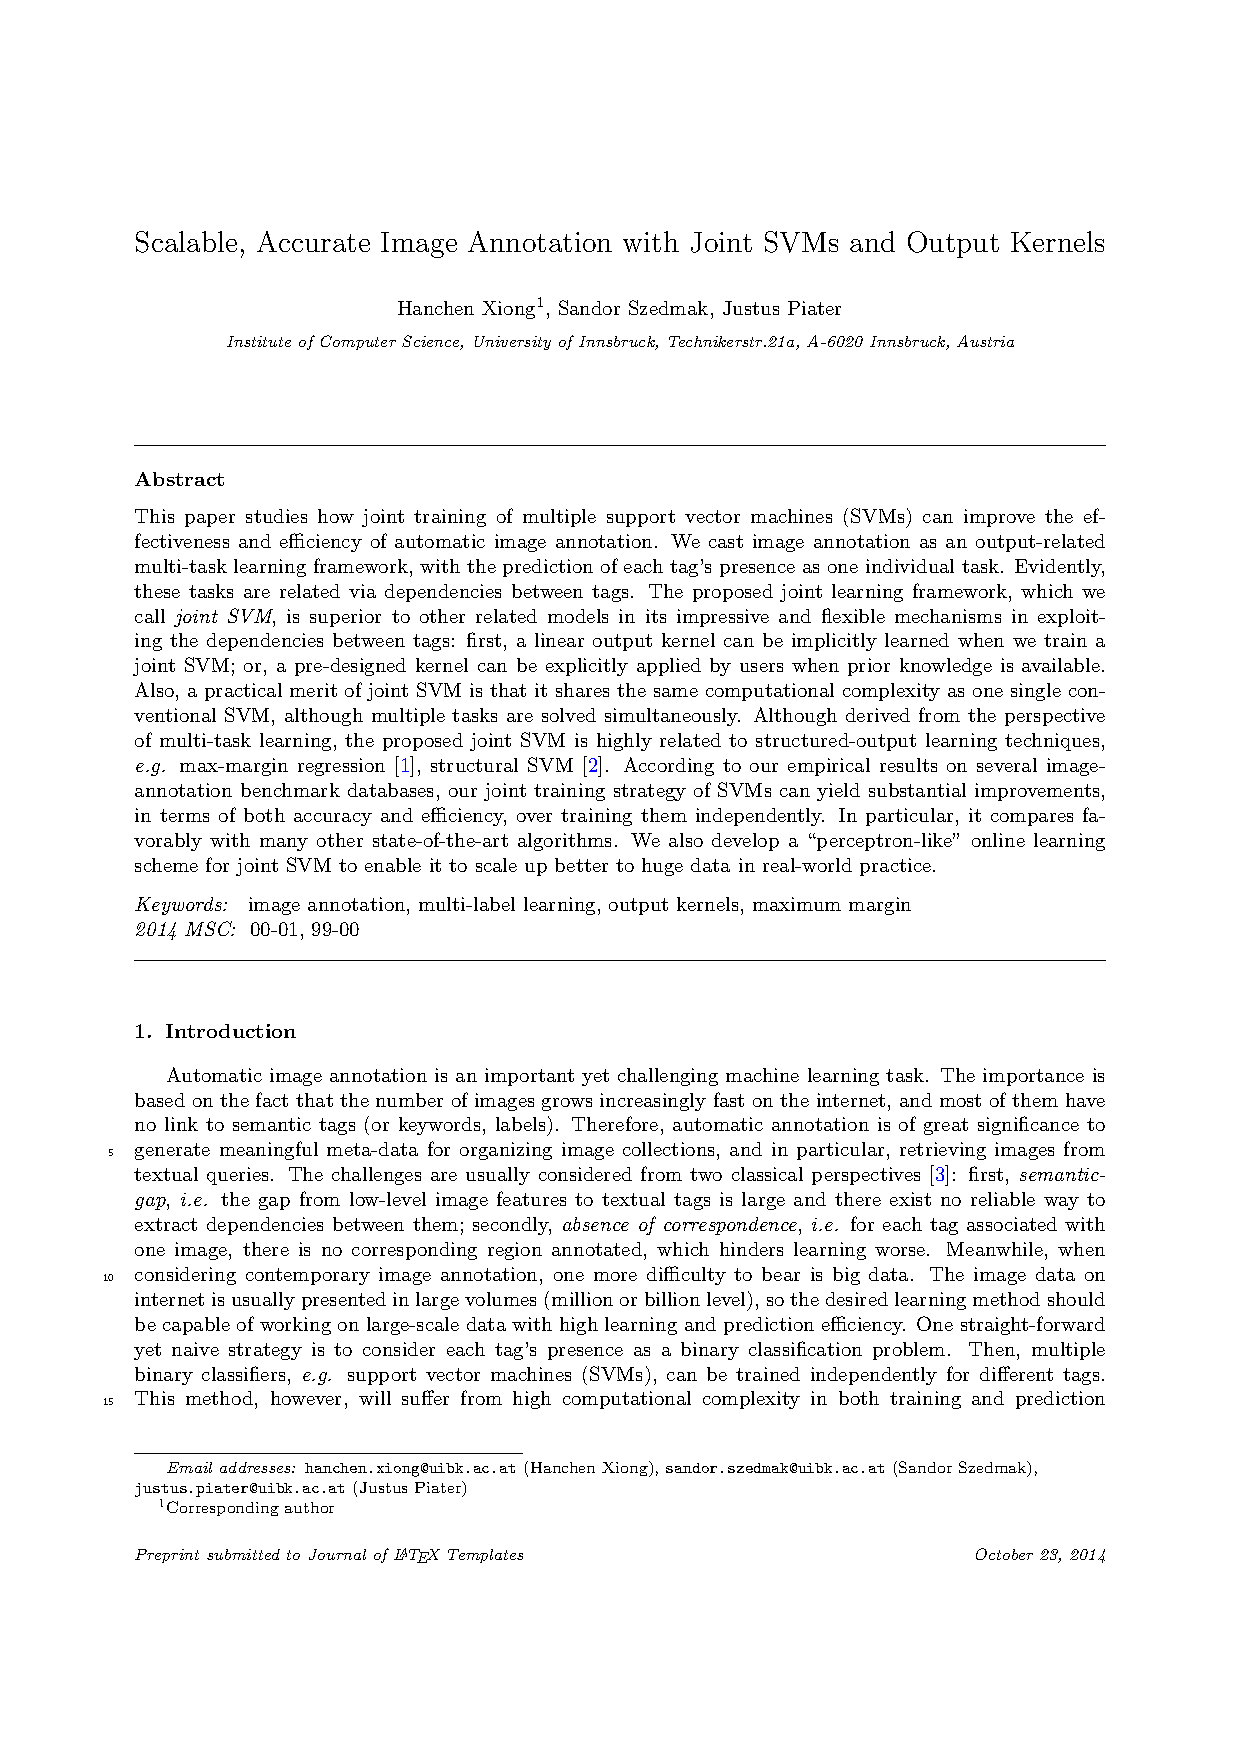
\includepdf[offset=3cm -2cm, scale=1, pages=-,pagecommand={\pagestyle{fancy}}]{./Papers/Xiong-2015-NEUCOM.pdf}
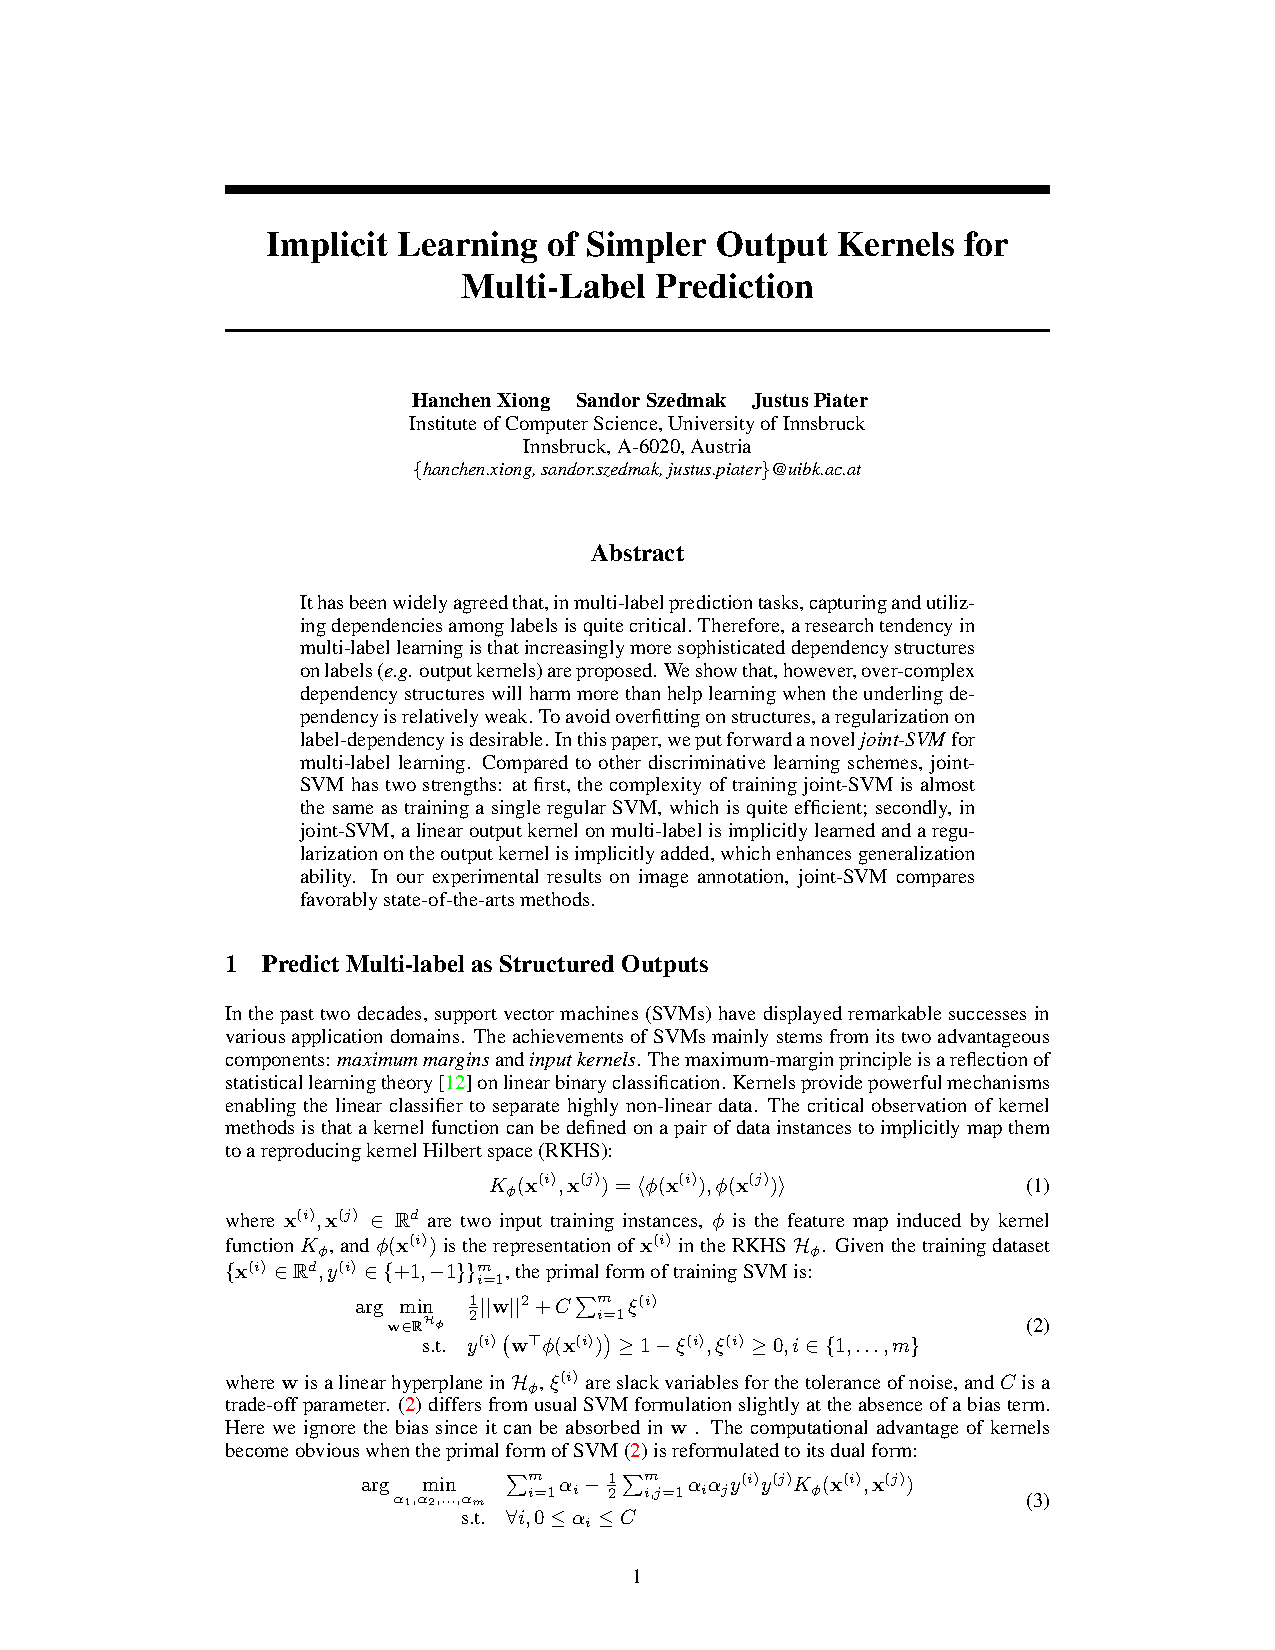
\includepdf[offset=3cm -2cm, scale=1, pages=-,pagecommand={\pagestyle{fancy}}]{./Papers/Xiong-2014-NIPS-RLCO.pdf}






%----------------------------------------------------------------------------------------
%	SECTION 2
%----------------------------------------------------------------------------------------
\section{Homogeneity Analysis for Object-Action Relation Learning}
\begin{shaded}
{\Huge VII.} \textbf{Hanchen Xiong}, Sandor Szedmak, Justus Piater {\it Homogeneity Analysis for Object-Action Relations Reasoning in Kitchen Scenarios}, 
In Proceedings of 2nd Workshop on Machine Learning for Intelligent Systems (MLIS13), pp 37-44,  2013, ACM. 
\vspace{-.2cm}
\end{shaded}

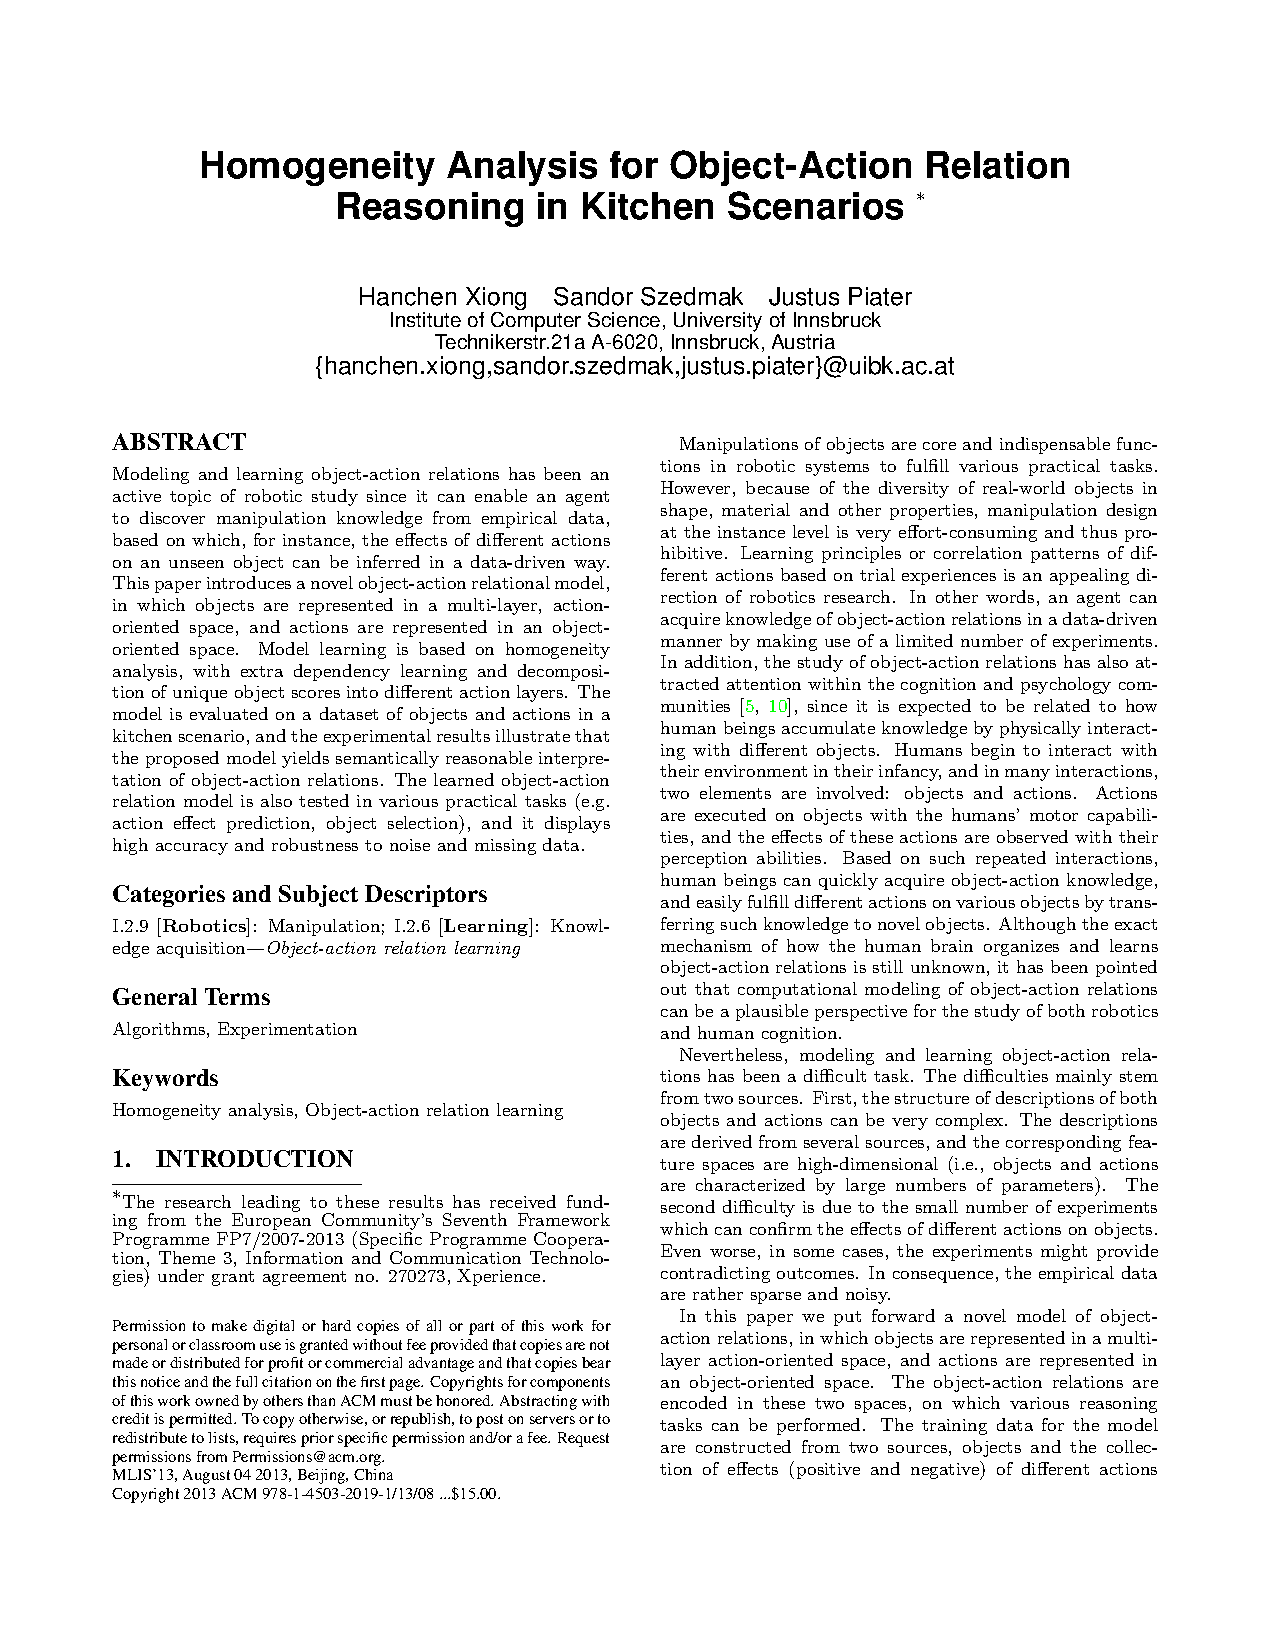
\includepdf[offset=3cm -3cm, scale=1, pages=-,pagecommand={\pagestyle{fancy}}]{./Papers/Xiong-2013-MLIS.pdf}

%----------------------------------------------------------------------------------------
%	SECTION 3
%----------------------------------------------------------------------------------------

\section{Multi-Label Learning with Kernel Generalized Homogeneity Analysis}
\begin{shaded}
 {\Huge X.} \textbf{Hanchen Xiong}, Sandor Szedmak, Justus Piater {\it Multi-Label Learning with Kernel Generalized Homogeneity Analysis}, 
Unpublished, 2015.
\end{shaded}

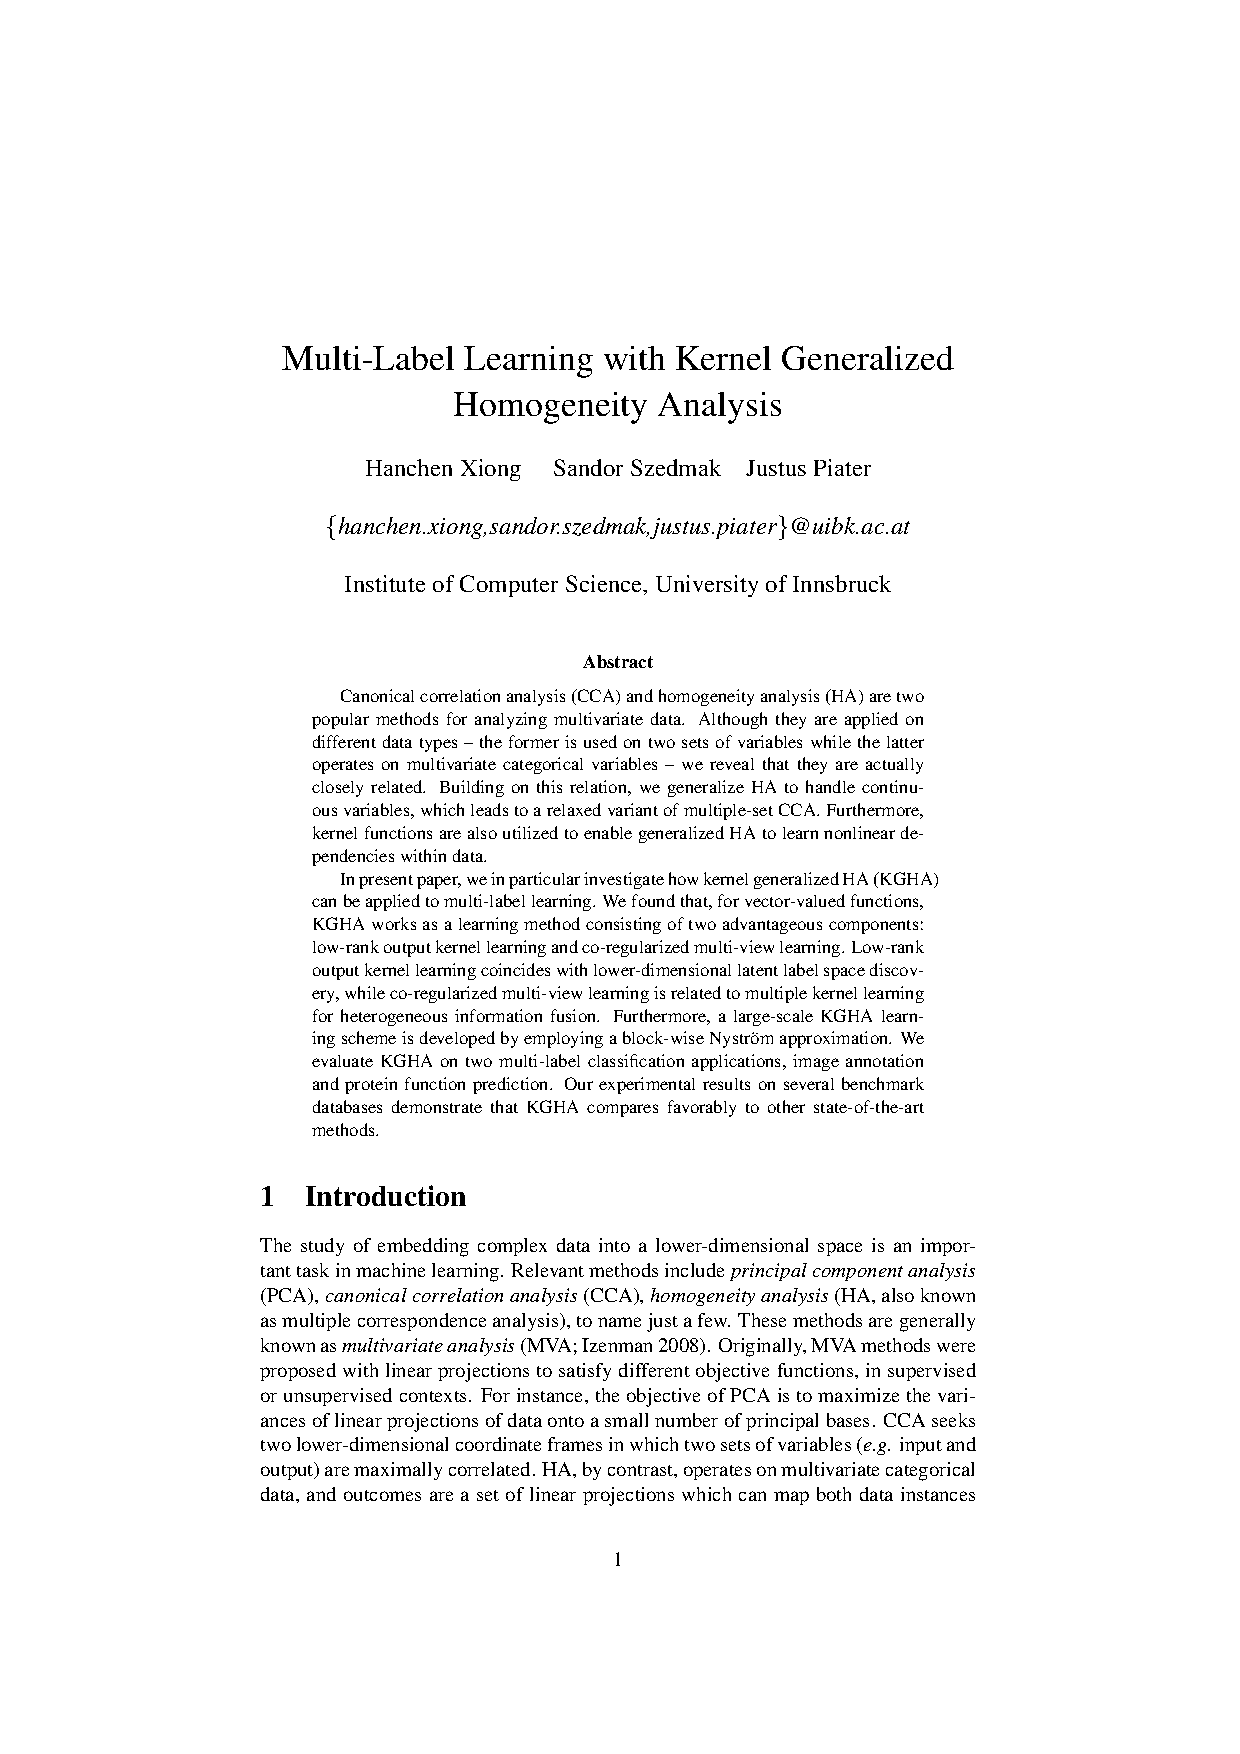
\includepdf[offset=3cm -3cm, scale=1.2, pages=-,pagecommand={\pagestyle{fancy}}]{./Papers/KGHA.pdf}

